% !TeX spellcheck = en_GB

\section{A Family of Multi-Compartment LIF Neurons}
\label{sec:nlif}

The dendritic nonlinearity $H$ introduced in the last section maps some channel state $\vec g$ onto an average somatic current.
While this mapping can always be established numerically, expressing $H$ in closed form has the potential to simplify the optimisation problem in \cref{eqn:decode_nonlinear_synapses}.

In this section, we discuss a family of multi-compartment \LIF neurons that we refer to as \enquote{$n$-LIF}.
These neurons are based on the multi-compartment neurons that we reviewed in \Cref{sec:comp}, and, as we discussed in the introduction of this chapter, were constructed with mathematical tractability in mind, rather than biological detail.
While it is not possible to derive an exact dendritic nonlinearity $H$ for these neurons, we derive a closed-form \enquote{surrogate} model of $H$ that can be fit to numerical data.

\subsection{Mathematical Description of $n$-LIF Neurons}
\label{sec:nlif_description}

\begin{figure}
	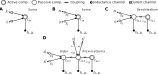
\includegraphics{media/chapters/03_nlif/03_03/multi_compartment_examples.pdf}%
	{\phantomsubcaption\label{fig:nlif_a}}%
	{\phantomsubcaption\label{fig:nlif_b}}%
	{\phantomsubcaption\label{fig:nlif_c}}%
	{\phantomsubcaption\label{fig:nlif_d}}%
	{\phantomsubcaption\label{fig:nlif_e}}%
	\caption[\enquote{Ball-and-stick} illustration of multi-compartment LIF neurons]{\enquote{Ball-and-stick} illustration of multi-compartment \LIF neurons.
	Large circles correspond to compartments, small circles and rectangles to conductance- and current-based channels. Filled symbols indicate passive channels.
	\textbf{(A)} Standard \LIF neuron with current-based inputs.
	\textbf{(B)} \LIF neuron with conductance-based input channels.
	\textbf{(C)} Two-compartment neuron with a separate dendritic compartment.
	\textbf{(D, E)} Three- and four-compartment \LIF neurons with apical and basal dendrites.}
	\label{fig:nlif}
\end{figure}

We define an \nlif neuron as a connected graph of resistively coupled capacitive compartments.
Each neuron possesses exactly one active compartment with standard \LIF dynamics, while the other compartments represent a passive dendritic tree.
Each compartment may hold any number of passive current- and conductance-based channels.
Channels are either constant (representing bias currents and leak channels), or receive external input (representing synapses).
Examples of such neurons are depicted in \Cref{fig:nlif} using a \enquote{ball-and-stick} representation.

As a point of reference, the expanded equivalent circuit diagram of the two-compartment neuron with conductance-based synapses (\Cref{fig:nlif_c}) is depicted in \Cref{fig:two_comp_lif_circuit}.
This particular model has originally been described by \citet{vu1993mechanism} and was subsequently discussed by \citet{koch1999biophysics} and \citet{capaday2006direct}.
We discuss this model in more detail in the next section, and for now focus on \nlif neurons in general.

\begin{figure}
	\includegraphics{media/chapters/03_nlif/03_03/neuron_model_trace_composite.pdf}%
	{\phantomsubcaption\label{fig:two_comp_lif_circuit}}
	{\phantomsubcaption\label{fig:two_comp_lif_trace}}
	\caption[Circuit and membrane potential trace of a two-compartment LIF neuron]{Circuit and membrane potential trace of a two-compartment neuron.
	\textbf{(A)} Circuit diagram corresponding to the model in \Cref{fig:nlif_c}.
	\textbf{(B)} Membrane potential traces for both compartments for a small constant excitatory input.
	Notice how the explicit spike model in the somatic compartment (\emph{top}) influences the membrane potential of the dendritic compartment (\emph{bottom}).}
	\label{fig:two_comp_lif}
\end{figure}

\subsubsection{Superthreshold dynamics}
In contrast to the standard \LIF model (cf.~\Cref{sec:simplified_neuron_models}), the active \nlif compartment possess an explicit spike model.
As pointed out by \citet{capaday2006direct}, this is important in multi-compartment models, since the spike potential causes a substantial current to backpropagate into the dendritic compartments (cf.~\Cref{fig:two_comp_lif_trace}).

More precisely, we model the superthreshold dynamics as follows.
Whenever the membrane potential \vMem surpasses the threshold $v_\mathrm{th}$, \vMem is clamped to a \enquote{spike potential} $v_\mathrm{spike}$ for a period $\tau_\mathrm{spike}$ and subsequently forced to $v_\mathrm{reset}$ for the refractory period $\tau_\mathrm{ref}$.
Unless specified otherwise, we use $\tau_\mathrm{spike} = \SI{1}{\milli\second}$ and $\tau_\mathrm{ref} = \SI{2}{\milli\second}$ in our models.

\subsubsection{Subthreshold dynamics}
The dynamics of the $i$th compartment are
\begin{align}
	\Cmi \frac{d}{dt} \vMemi(t) &=
		\sum_{k=1}^{M_i} g_k^i(t) \bigl( E_k^i - \vMemi(t) \bigr) +
		\sum_{k=1}^{N_i} J_k^i(t) +
		\sum_{j=1}^{n} \bigl(\vMemj(t) - \vMemi(t)\bigr) \cij \,,
\label{eqn:nlif_single_compartment}
\end{align}
where \Cmi is the membrane capacitance of the compartment, $M_i$ and $N_i$ are the number of conductance- and current-based channels, respectively, $g_{k}^i(t)$ is the momentary conductance of the $k$th conductance-channel with reversal potential $E_{k}^i$, and $J_{k}^i(t)$ is the current injected into the current-based channel $j$.
Finally, \cij is the coupling conductance between the $i$th and the $j$th compartment.
The adjacency matrix of coupling conductances $\mat C$ must be symmetric, and the connectivity graph encoded by $\mat C$ must have exactly one connected component (cf.~our discussion in \Cref{sec:comp}).
Some conductances $g_{k}^i(t)$ and currents $J_{k}^i(t)$ are constant, such as the static leak channels and bias currents.

\begin{table}
	\caption[Matrix representations of the first four neuron models in \Cref{fig:nlif}]{Matrix representations of the first four neuron models in \Cref{fig:nlif}. See text for details.
	%All matrices are multiplied by the membrane capacitance $C_\mathrm{m}$ (assuming that $C_\mathrm{m}$ is the same across compartments).
	}
	\label{tbl:nlif_matrices}
	\small\sffamily\centering
	\begin{tabular}{c c c c c c}
		\toprule
		\multicolumn{1}{c}{\textbf{Model}} & \vnap & \mnAp & \vnbp & \mnBp & \mnL \\
		\midrule
		%\cmidrule{1-1}\cmidrule(l){2-6}
			\textbf{(A)}
			& $\displaystyle \begin{bmatrix} g_\mathrm{L} \end{bmatrix}$
			& $\displaystyle \begin{bmatrix} 0 & 0 \end{bmatrix}$
			& $\displaystyle \begin{bmatrix} g_\mathrm{L} E_\mathrm{L} \end{bmatrix}$
			& $\displaystyle \begin{bmatrix} 1 & -1 \end{bmatrix}$
			& $\displaystyle \begin{bmatrix} 0 \end{bmatrix}$\\[0.5cm]
			\textbf{(B)} 
			& $\displaystyle \begin{bmatrix} g_\mathrm{L} \end{bmatrix}$
			& $\displaystyle \begin{bmatrix} 1 & 1 \end{bmatrix}$
			& $\displaystyle \begin{bmatrix} g_\mathrm{L} E_\mathrm{L} \end{bmatrix}$
			& $\displaystyle \begin{bmatrix} E_\mathrm{E} & E_\mathrm{I} \end{bmatrix}$
			& $\displaystyle \begin{bmatrix} 0 \end{bmatrix}$ \\[0.5cm]
			\textbf{(C)} 
			& $\displaystyle \begin{bmatrix}
				g_\mathrm{L} \\ g_\mathrm{L}
			\end{bmatrix}$
			& $\displaystyle \begin{bmatrix} 0 & 0 \\
				1 & 1 \end{bmatrix}$
			& $\displaystyle \begin{bmatrix}
				g_\mathrm{L} E_\mathrm{L} \\
				g_\mathrm{L} E_\mathrm{L}
			\end{bmatrix}$
			& $\displaystyle \begin{bmatrix}
				0 & 0 \\
				E_\mathrm{E} & E_\mathrm{I}
			\end{bmatrix}$
			& $\displaystyle \begin{bmatrix} c_{12} & -c_{12} \\ -c_{12} & c_{12} \end{bmatrix}$ \\[0.5cm]
			\textbf{(D)} 
			& $\displaystyle \begin{bmatrix}
				g_\mathrm{L} \\
				g_\mathrm{L} \\
				g_\mathrm{L}
			\end{bmatrix}$
			& $\displaystyle \begin{bmatrix}
			    0 & 0 & 0 & 0\\
				1 & 1 & 0 & 0 \\
				0 & 0 & 1 & 1 \end{bmatrix}$
			& $\displaystyle \begin{bmatrix}
				g_\mathrm{L} E_\mathrm{L} \\
				g_\mathrm{L} E_\mathrm{L} \\
				g_\mathrm{L} E_\mathrm{L}
			\end{bmatrix}$
			& $\displaystyle \begin{bmatrix}
				0 & 0 & 0 & 0 \\
				E_\mathrm{E} & E_\mathrm{I} & 0 & 0 \\
				0 & 0 & E_\mathrm{E} & E_\mathrm{I} \\
			\end{bmatrix}$
			& $\displaystyle \begin{bmatrix} c_{12} & -c_{12} & 0 \\ -c_{12} & c_{12} + c_{23} & -c_{23} \\ 0 & -c_{23} & c_{23} \end{bmatrix}$ 			\\
		\bottomrule
	\end{tabular}
\end{table}

\subsubsection{Canonical matrix form}
We can rearrange \cref{eqn:nlif_single_compartment} to \emph{resemble} a canonical \LTI system.%
\footnote{
In general, \cref{eqn:nlif_matrix} is \emph{not} a linear dynamical system.
However, there are two conditions under which this system is linear: either $\vng(t)$ is constant, or there are no product terms between $\vng(t)$ and $\vvMem(t)$.
This is the case if the system has no conductance-based input channels and \mnAp is zero.
Note that the constant offset \vnbp in \cref{eqn:nlif_matrix} does not make the dynamical system nonlinear, but merely mandates one auxiliary dimension.
}
Let $k$ be the number of non-static input channels, and $\vng \in \mathbb{R}^k$ a vector representing all input channel states, that is, all non-static conductances $g_{ij}$ and currents $J_{ij}$.
This channel state is generally linear in the synaptic weights and the pre-activities (cf.~\Cref{sec:nef_nonlinear}).
We have
\begin{align}
	\frac{\mathrm{d}}{\mathrm{d}t} \vCm \circ \vvMem(t)
	&= \mnA\bigl[\vng(t)\bigr] \vvMem(t) + \vnb\bigl[\vng(t)\bigr]
	 = -\bigl[\mnL + \mathrm{diag}\bigl(\vnap + \mnAp \vng(t)\bigr)\bigr] \vvMem(t) + \big[\vnbp + \mnBp \vng(t)\big] \,.
	\label{eqn:nlif_matrix}
\end{align}
Here, $\vCm \in \mathbb{R}^n$ is a vector of membrane capacitances, \enquote{$\circ$} denotes elementwise multiplication, $\mnA[\vng(t)] \in \mathbb{R}^{n \times n}$ is the \enquote{voltage feedback matrix}, and $\vnb[\vng(t)] \in \mathbb{R}^n$ describes the input to the system.
We further decompose \mnA, \vnb into input-independent and input-dependent terms.
The Laplacian $\mnL \in \mathbb{R}^{n \times n}$ and the vectors $\vnap \in \mathbb{R}^n$, $\vnbp \in \mathbb{R}^n$ describe the input-independent portions of the system, whereas the matrices $\mnAp \in \mathbb{R}^{n \times k}$ and $\mnBp \in \mathbb{R}^{n \times k}$ describe its input-dependent parts.

More specifically, the Laplacian \mnL is the difference between the weighted degree matrix and the adjacency matrix, and, in our case, is given as $\mnL = \diag(\mC \mat I) - \mC$.%
\footnote{Indeed, the graph Laplacian is often motivated in textbooks with electrical networks similar to the one discussed here; in this context, it is also referred to as the \enquote{Kirchhoff matrix} \citep[e.g.,][Chapter~2]{bollobas1998modern}.}
The vector \vnap consists of sums of static channel conductances for each channel (such as the leak conductance) and \vnbp contains the sums of the static channel conductances multiplied by their reversal potential.
The matrix \mnAp contains one-entries for input-variables influencing a conductance-based channel in the corresponding compartment.
\mnBp contains a \enquote{one} for each variable current-based channel in the corresponding compartment, and the reversal potential for each variable conductance-based channel in a compartment.
Examples of these matrices for the first four \nlif neuron models depicted in \Cref{fig:nlif} are given in \Cref{tbl:nlif_matrices}.

\pagebreak

\subsection{Analysis of the Subthreshold $n$-LIF Dynamics}
\label{sec:nlif_subth_properties}

The dynamics of the \nlif system are quite benign.
The system is generally stable and does not oscillate; in other words, the eigenvalues of $\mnA[\vng] \diag(\vCm)^{-1}$ are real-valued and strictly negative \citep[e.g.,][Chapter~5]{strogatz1994nonlinear}.
More formally (see \Cref{app:thm_nlif_convergence} for a proof):
\begin{restatable}{theorem}{ThmNlifConvergence}
\label{thm:nlif_convergence}
Consider an $n$-LIF neuron with at least one static conductance-based channel and any input vector \vng with nonnegative entries for conductance-based input channels.
In this case, the feedback matrix $\mnA[\vng] \diag(\vCm)^{-1}$ is negative definite for any constant input vector $\vng$.
\end{restatable}
This is quite intuitive from a physical perspective.
The \nlif neuron is a resistor-capacitor network.
When tying at least one point of the network to a voltage source, the potential over the capacitors converges to an equilibrium $\vneq$.
For constant \vng the dynamics are
\begin{align}
	{\vMem}(t)
		&= \vneq + \exp\big(\mnA[\vng] \diag(\vCm)^{-1} t\big) \big(\vvMem(0) - \vneq\big) \,,
		& \text{where }  \vneq &= -\mnA[\vng]^{-1} \vnb[\vng] \,,
	\label{eqn:nlif_dynamics}
\end{align}
Crucially, $\mnA[\vng]$ is guaranteed to be invertible under the conditions listed in \Cref{thm:nlif_convergence}.
%It is singular exactly if the neuron does not possess any conductance-based channels, or the conductances of all channels are zero.
Furthermore, note that \vneq does not depend on \vCm; both $\mnA[\vng]$ and $\vnb[\vng]$ are divided by \vCm (cf.~eq.~\ref{eqn:nlif_matrix}):
\begin{align*}
	  \bigl(\diag(\vCm)^{-1} \mnA[\vng]\bigr)^{-1} \bigl(\diag(\vCm)^{-1} \vnb[\vng]\bigr)
	= \mnA[\vng]^{-1} \diag(\vCm) \diag(\vCm)^{-1} \vnb[\vng] = \mnA[\vng]^{-1} \vnb[\vng] \,.
\end{align*} 

\begin{figure}
	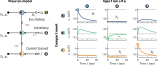
\includegraphics{media/chapters/03_nlif/03_03/nlif_impulse_response_panels.pdf}
	\caption[Impulse response of the $n$-LIF neuron]{Impulse response of the $n$-LIF neuron.
	Injecting a pulse into a nonlinear conductance channel (injection sites \emph{1}, \emph{2}) at most charges the corresponding compartment up to the channel reversal potential.
	In contrast, current inputs (injection site \emph{3}) can charge the membrane to arbitrary potentials.
	The impulse is filtered and dampened while it is travelling through a neuron.
	}
	\label{fig:nlif_impulse_response_panels}
\end{figure}
The impulse response of the system is depicted in \Cref{fig:nlif_impulse_response_panels}.
Each compartment acts as a first-order low-pass filter; the response in compartment $i$ to an impulse in compartment $j$ thus resembles a low-pass filter of order $d(i, j)$, the distance between nodes $i$, $j$.
%However, once again note that conductance channels are nonlinear---the impulse response does not fully characterise the system.
%No matter what the previous membrane potential, an input will at most charge the corresponding compartment up to the channel reversal potential.

\subsection{Deriving a Surrogate Model of the Dendritic Nonlinearity $H$}
\label{sec:nlif_derive_h}

As defined above (cf.~\Cref{def:dendritic_nonlinearity}), the dendritic nonlinearity $H$ maps a synaptic state $\vec g$ onto the synaptic current $J$ such that $G[J] = \mathscr{G}[\vec g]$, where $G[J]$ is a standard single-channel response curve and $\mathscr{G}[\vec g]$ is the response curve of the multi-channel neuron.
If, for example, $G[J]$ is the \LIF response curve, then $H$ maps $\vec g$ into an \enquote{\LIF-equivalent} current.

Trivial cases aside, it is generally not possible to provide $H$ in closed form for \nlif neurons.
This is due to the nonlinear interaction between the membrane potential and conductance-based input channels, as well as the influence of the nonlinear superthreshold dynamics on the dendritic compartments.
Still, we can derive a parametrised \enquote{surrogate model} that approximates $H$ well and that we can fit to empirical data.

\subsubsection{Subthreshold current}
As a first step towards this model, consider the case where the neuron model is purely in its subthreshold regime.
Without loss of generality, assume that the compartment with index $i = 1$ is the somatic compartment.
Furthermore, assume that this compartment possesses a leak channel with conductance $g_\mathrm{L}$ and reversal potential $E_\mathrm{L}$.
The current $H(\vec g; t)$ flowing into the somatic compartment at time $t$ for constant $\vec g$ is the differential of $v_1$ divided by the membrane capacitance, that is
\begin{align}
	H(\vec g; t) = \big(\mat A[\vec g] \vec v(t) + \vec b[\vec g] \big)_1 \,.
	\label{eqn:nlif_sub_momentary}
\end{align}
To obtain a \LIF-equivalent current, we must further subtract the leak current $g_\mathrm{L} \big( E_\mathrm{L} - v_1(t) \big)$; this current is already accounted for in the \LIF response curve $G[J]$.%
\footnote{
Of course, $H$ depends on the specific choice of $G[J]$.
For example, if we used the response curve for an non-leaky IF-neuron instead, we would not have to subtract the leak current.
More specifically, in the next section, we discuss using a rectified linear unit instead of the \LIF response curve.
Also note that, in practice, these details are not too critical.
As we discuss below, we propose using a parametrised version of $H$ that is fit to numerical measurements of $J$; this process naturally compensates for missing offsets.
}

\begin{figure}[p]
	\centering
	\includegraphics{media/chapters/03_nlif/03_03/average_som_pot.pdf}%
	{\phantomsubcaption\label{fig:avg_vsom_a}}%
	{\phantomsubcaption\label{fig:avg_vsom_b}}%
	\caption[Mean somatic membrane potential over the neuron output rate]{Mean somatic membrane potential $\vSom$ over the output rate for a current-based \LIF neuron. Lines correspond to the average potential for different pre-synaptic spike rates.
	Mean post-synaptic currents are fixed in individual trials, so the spike rate purely corresponds to the amount of noise.
	Data over 128 random Poisson spike-trains per 1000 individual mean post-synaptic currents.
	Synaptic filter time-constant is $5\,\mathrm{ms}$. Shaded areas correspond to 25/75\% percentiles, lines to the mean.
	\textbf{(A)} Average membrane potential including the refractory and spike period.
	\textbf{(B)} Average membrane potential excluding the refractory and spike period. Dotted line is a  linear model that takes the relative length of the spike and refractory phase into account.}
	\label{fig:avg_vsom}
\end{figure}

\begin{table}[p]
	\caption[Reduced matrix representations of the first four neuron models in \Cref{fig:nlif}]{Reduced matrix representations of the first four multi-compartment neuron models in \Cref{fig:nlif}.
	The somatic compartment is disconnected from the remaining neuron model.
	Connections to the somatic compartment are replaced by a static conductance-based channel with reversal potential $\vSom$. The voltage difference between $\vSom$ and the equilibrium potential of the new model is proportional to the current flowing into the somatic compartment.
	}
	\label{tbl:nlif_matrices_reduced}
	\small\sffamily\centering
	\begin{tabular}{c c c c c c c}
		\toprule
		\multicolumn{1}{c}{\textbf{Model}\!\!} & $\vec{\tilde a}'$ & $\mat{\tilde A}'$ & $\vec{\tilde b}'$ & $\mat{\tilde B}'$ & $\mat{\tilde L}$ & $\vec{\tilde c}$\\
		\midrule
			\textbf{(A)}
			& $\displaystyle \begin{bmatrix} 1 \end{bmatrix}$
			& $\displaystyle \begin{bmatrix} 0 & 0 \end{bmatrix}$
			& $\displaystyle \begin{bmatrix} g_\mathrm{L} ( E_\mathrm{L} - \vSom ) + \vSom \end{bmatrix}$
			& $\displaystyle \begin{bmatrix} 1 & -1 \end{bmatrix}$
			& $\displaystyle \begin{bmatrix} 0 \end{bmatrix}$
			& $\displaystyle \begin{bmatrix} 1 \end{bmatrix}$\\[0.5cm]
			\textbf{(B)}
			& $\displaystyle \begin{bmatrix} 1 \end{bmatrix}$
			& $\displaystyle \begin{bmatrix} 0 & 0 \end{bmatrix}$
			& $\displaystyle \begin{bmatrix} g_\mathrm{L} ( E_\mathrm{L} - \vSom ) + \vSom \end{bmatrix}$
			& $\displaystyle \begin{bmatrix} E_\mathrm{E} - \vSom & E_\mathrm{I} - \vSom \end{bmatrix}$
			& $\displaystyle \begin{bmatrix} 0 \end{bmatrix}$
			& $\displaystyle \begin{bmatrix} 1 \end{bmatrix}$\\[0.5cm]
			\textbf{(C)}
			& $\displaystyle \begin{bmatrix}
				1 \\
				g_\mathrm{L} + c_\mathrm{12}
			\end{bmatrix}$
			& $\displaystyle \begin{bmatrix}
				0 & 0 \\
				1 & 1 \end{bmatrix}$
			& $\displaystyle \begin{bmatrix}
				g_\mathrm{L} ( E_\mathrm{L} - \vSom ) + \vSom \\
				g_\mathrm{L} E_\mathrm{L} + c_{12} \vSom
			\end{bmatrix}$
			& $\displaystyle \begin{bmatrix}
				0 & 0 \\
				E_\mathrm{E} & E_\mathrm{I}
			\end{bmatrix}$
			& $\displaystyle \begin{bmatrix} 0 & 0 \\ 0 & 0 \end{bmatrix}$
			& $\displaystyle \begin{bmatrix} 1 \\ c_{12} \end{bmatrix}$\\[0.5cm]
			\textbf{(D)} 
			& $\displaystyle \begin{bmatrix}
				1 \\
				g_\mathrm{L} + c_\mathrm{12}\\
				g_\mathrm{L}
			\end{bmatrix}$
			& $\displaystyle \begin{bmatrix}
				0 & 0 & 0 & 0 \\
				1 & 1 & 0 & 0 \\
				0 & 0 & 1 & 1 \end{bmatrix}$
			& $\displaystyle \begin{bmatrix}
				g_\mathrm{L} ( E_\mathrm{L} - \vSom ) + \vSom \\
				g_\mathrm{L} E_\mathrm{L} + c_{12} \vSom \\
				g_\mathrm{L} E_\mathrm{L}
			\end{bmatrix}$
			& $\displaystyle \begin{bmatrix}
				0 & 0 & 0 & 0 \\
				E_\mathrm{E} & E_\mathrm{I} & 0 & 0 \\
				0 & 0 & E_\mathrm{E} & E_\mathrm{I} \\
			\end{bmatrix}$
			& $\displaystyle \begin{bmatrix}
				0 & 0 & 0 \\
				0 & c_{23} & -c_{23} \\
				0 & -c_{23} & c_{23} \end{bmatrix}$
			& $\displaystyle \begin{bmatrix} 1 \\ c_{12} \\ 0 \end{bmatrix}$\\
		\bottomrule
	\end{tabular}
\end{table}

\subsubsection{Average superthreshold somatic potential}
For the purpose of building networks of spiking neurons, we are primarily interested in the superthreshold regime.
Unfortunately, as mentioned above, the nonlinear superthreshold dynamics are notoriously difficult to analyse.

We work around this by exploiting the fact that \nlif neurons are tonically spiking (cf.~\Cref{sec:simplified_neuron_models}).
That is, the somatic compartment oscillates between the reset and threshold potential with a fixed frequency (cf.~\Cref{fig:izhikevich_whichmod_figure1}).
We may thus assume that the somatic membrane potential is effectively clamped to some value $\vSom$ between reset and threshold potential; we discuss this in more detail in \citet{stockel2017point}.

As is depicted in \Cref{fig:avg_vsom}, this assumption is reasonable for a wide range of output rates, as long as we ignore the spike and refractory period.
This latter simplification is justified, since due to clamping, the current flowing into the somatic compartment during these periods has no direct influence on the output rate of the neuron.
Of course, in multi-compartment models, there is the smaller, indirect effect of the somatic membrane potential influencing the state of the dendritic compartments, but we ignore this for now.

\subsubsection{Average somatic current}
To estimate the average current flowing into the somatic compartment, we replace the system from \cref{eqn:nlif_matrix} with a reduced system with vectors and matrices $\vec{\tilde a}'$, $\vec{\tilde b}'$, $\mat{\tilde A}'$, $\mat{\tilde B}'$, and $\mat{\tilde L}'$.
These matrices describe a dynamical system of the form%
\begin{align}
	\frac{\D}{\D t} \vec{\tilde C}_\mathrm{m} \circ \vec{\tilde v}(t)
	&= \mat{\tilde A}\big[\vec g(t)\big] \vec{\tilde v}(t) + \vec{\tilde b}\big[\vec g(t)\big]
	 = -\big[\mat{\tilde L} + \mathrm{diag}\big(\vec{\tilde a'} + \mat{\tilde A'} \vec g(t)\big)\big] \vec v(t) + \big[\vec{\tilde b}' + \mat{\tilde B}' \vec g(t)\big] \,.
	\label{eqn:nlif_matrix_reduced}
\end{align}
For constant $\vec g$, this system is linear and, analogously to what we have discussed in \Cref{sec:nlif_subth_properties}, converges to an equilibrium state $\vec {\tilde v}^\mathrm{eq}$:
\begin{align}
	\vec{\tilde v}(t)
	=
	  \vec{\tilde v}^\mathrm{eq}
	+ \exp\bigl(
		\mat{\tilde A}[\vec g] \diag(\vec{\tilde C}_\mathrm{m})^{-1} t
	  \bigr) \bigl(
	    \vec{\tilde v}(0) - \vec{\tilde v}^\mathrm{eq}
	  \bigr) \,,
	\quad\quad \text{where} \quad \vec{\tilde v}^\mathrm{eq} &= -{\mat{\tilde A}}[\vec g]^{-1} \vec{\tilde b}[\vec g] \,.
	\label{eqn:nlif_eq}
\end{align}

This reduced system is constructed such that, for non-somatic compartments, the equilibrium potential $\vec{\tilde v}^\mathrm{eq}$ converges to the voltage that we would obtain if the somatic compartment were clamped to \vSom.
In the somatic compartment itself, the voltage difference $\tilde v^\mathrm{eq}_1 - \vSom$ is proportional to the current flowing into the compartment.
Given a vector $\vec{\tilde c}$ of somatic coupling conductances with $\tilde c_1 = 1$, the average current $H(\vec g)$ flowing into the soma is then modelled as
\begin{align}
	H(\vec g) &= \lim_{T \to \infty} \frac{1}T \int_{0}^T H(\vec g; t) \,\D t \approx \sum_{i = 1}^n \tilde c_i (\tilde v^\mathrm{eq}_i - \vSom) \,.
	\label{eqn:h_model}
\end{align}

In practice, we obtain the reduced system by setting the first column and row of $\mat{\tilde L}$ to zero and replacing connections to the somatic compartment with static conductance-based channels.
In the somatic compartment, all conductance-based channels are replaced by current-based channels weighted by the difference between $\vSom$ and the channel reversal potential (cf.~\cite{stockel2017point}); furthermore, we let $(\vec {\tilde a}')_1 = 1$ and add $\vSom$ to $(\vec {\tilde b'})_1$.
We provide examples of reduced systems in \Cref{tbl:nlif_matrices_reduced}.

As a word of warning, note that the reduced system as described here is conceptually useful, but notoriously ill-conditioned. 
We address this in \Cref{app:nlif_conditioning} by rescaling and offsetting the system such that $\mat{\tilde A}[\vec g]^{-1} \vec{\tilde b}[\vec g]$ directly represents currents instead of voltages.

\subsubsection{Model parameters}
\Cref{eqn:h_model} is the result of major simplifications and as such unlikely to be accurate.
Specifically, we assumed that the somatic compartment is effectively clamped to a constant potential $\vSom$, that $\vec g$ is constant, and that spike generation has no effect on the dendritic compartments.
These assumptions are readily violated in practice.
The average somatic potential $\vSom$ depends on the pre-synaptic noise-level (cf.~\Cref{fig:avg_vsom}), the input $\vec g$ is seldom constant, and spike generation affects the dendritic membrane potentials (cf.~\Cref{fig:two_comp_lif_trace}).

Thus, equation~(\ref{eqn:h_model}) is better interpreted as a \enquote{template} for the overall mathematical shape of the dendritic nonlinearity.
That is, to at least partially compensate for the imprecisions in our derivation, we declare $\vec{\tilde a}'$, $\vec{\tilde b}'$, as well as the non-zero entries in $\mat{\tilde A}'$, $\mat{\tilde B}'$ to be free parameters.
Keeping the graph Laplacian $\mat{\tilde L}$ and the zeros in $\mat{\tilde A'}$, $\mat{\tilde B'}$ fixed implies that we assume that the connectivity graph accurately describes the electrical network of the neuron.

%Note that this parametrisation is not minimal, in the sense that it does not have the least possible number of degrees of freedom.

The model parameters can be initialised with the original model and fit to direct numerical measurements of the somatic current $J$, or, alternatively, currents reconstructed from the neural activity, i.e., $J = G^{-1}[\mathscr{G}(\vec g)]$.
The calibration samples should be obtained from a setting that resembles the network context in which the neuron is used.
For example, the pre-synaptic noise level should match what the neuron would be exposed to in the network.

We discuss methods for determining the model parameters, and test the quality of $H$ in the following sections.
However, before we do so, we explicitly derive $H$ for a few special cases and analyse this dendritic nonlinearity model from a more theoretical perspective.


\subsection{Some Worked Examples}
\label{sec:nlif_examples}

The above framework is well-suited for algorithmically deriving the dendritic nonlinearity model $H$ for arbitrary \nlif neurons.
Unfortunately, it may be less intuitive when manually analysing these models.
%We can easily construct the corresponding model matrices and predict the somatic current for a given input configuration.
Hence, we find it useful to at least provide the expanded dendritic nonlinearity $H$ for the first four models depicted in \Cref{fig:nlif}.

\subsubsection{Single-compartment LIF neuron with current-based input}
Expanding \cref{eqn:h_model} for the model depicted in \Cref{fig:nlif_a} using \Cref{tbl:nlif_matrices_reduced} yields 
\begin{align*}
	H(J_\mathrm{E}, J_\mathrm{I}) = J_\mathrm{E} - J_\mathrm{I} + g_\mathrm{L}(E_\mathrm{L} - \vSom) \,.
\end{align*}
This function is visualised in \Cref{fig:dendritic_nonlinearity_comparison_a}. To obtain the \LIF-equivalent current we subtract the leak current, as mentioned above.
Using the fully parameterised version of the equations, and renaming the parameters for better readability, we obtain the following affine model:
\begin{align*}
	H(J_\mathrm{E}, J_\mathrm{I}) &= \tilde b'_1 + \tilde B'_{1, 1} J_\mathrm{E} + \tilde B'_{1, 2} J_\mathrm{I} = b_0 + b_1 J_\mathrm{E} + b_2 J_\mathrm{I} \,.
\end{align*}

\begin{figure}
	\includegraphics{media/chapters/03_nlif/03_03/dendritic_nonlinearity_comparison.pdf}%
	{\phantomsubcaption\label{fig:dendritic_nonlinearity_comparison_a}}%
	{\phantomsubcaption\label{fig:dendritic_nonlinearity_comparison_b}}%
	{\phantomsubcaption\label{fig:dendritic_nonlinearity_comparison_c}}%
	{\phantomsubcaption\label{fig:dendritic_nonlinearity_comparison_d}}%
	\caption[Dendritic nonlinearity models $H$ for different $n$-LIF neurons]{Dendritic nonlinearity models $H$ for the \nlif neurons depicted in \Cref{fig:nlif}. Hatched regions correspond to subthreshold currents. Limits were chosen such that the spike onset is approximately on the diagonal of each plot.
	Parameters shared between all models: $g_\mathrm{L} = \SI{50}{\nano\siemens}$, $C_\mathrm{m} = \SI{1}{\nano\farad}$, $E_\mathrm{L} = \SI{-65}{\milli\volt}$, $E_\mathrm{E} = \SI{20}{\milli\volt}$, $E_\mathrm{I} = \SI{-75}{\milli\volt}$, $\vSom = \SI{-57.5}{\milli\volt}$.
	\textbf{(A, B)} Single-compartment neurons with current- and conductance-based synapses. Apart from scaling, the two models are equivalent.
	\textbf{(C)}~Two-compartment neuron with $c_\mathrm{12} = \SI{30}{\nano\siemens}$. The contour lines are still straight lines but no longer parallel due to shunting.
	\textbf{(D)} Slice through the response curve of a three-compartment \LIF neuron with $c_\mathrm{12} = \SI{40}{\nano\siemens}$, $c_\mathrm{23} = \SI{100}{\nano\siemens}$. The inputs $g_E^2 = \SI{95}{\nano\siemens}$ and $g_I^1 = \SI{20}{\nano\siemens}$ are kept constant. In contrast to the two-compartment neuron, the contour-lines are curved.
	}
\end{figure}


\subsubsection{Single-compartment LIF neuron with conductance-based input}
For \Cref{fig:nlif_b} we obtain
\begin{align*}
	H(g_\mathrm{E}, g_\mathrm{I}) = g_\mathrm{E} (E_\mathrm{E} - \vSom) + g_\mathrm{I} (E_\mathrm{I} - \vSom) + g_\mathrm{L}(E_\mathrm{L} - \vSom) \,.
\end{align*}
This function is illustrated in \Cref{fig:dendritic_nonlinearity_comparison_b}.
The fully parameterised version of the model is
\begin{align*}
	H(g_\mathrm{E}, g_\mathrm{I}) &= \tilde b'_1 + \tilde B'_{1, 1} g_\mathrm{E} + \tilde B'_{1, 2} g_\mathrm{I} = b_0 + b_1 g_\mathrm{E} + b_2 g_\mathrm{I} \,.
\end{align*}
This is the equivalent to the current-based neuron model.

Crucially, this is not just an artefact of our modelling framework, but indeed captures the behaviour of spiking neuron simulations well.
We discuss this in more detail in \citet{stockel2017point}.
Independent experiments by \citet{kiselev2020approximating} further support this observation.
Hence, single-compartment \LIF neurons with conductance-based synapses are rather uninteresting from a computational perspective.

\subsubsection{Two-compartment LIF neuron}
For the model depicted in \Cref{fig:nlif_c} we have
\begin{align}
	H(g_\mathrm{E}, g_\mathrm{I}) = c_{12} \left(\frac{\vSom c_\mathrm{12} + E_\mathrm{L} g_\mathrm{L} + E_\mathrm{E} g_\mathrm{E} + E_\mathrm{I} g_\mathrm{I}}{c_\mathrm{12} + g_\mathrm{L} + g_\mathrm{E} + g_\mathrm{I}} - \vSom \right) + g_\mathrm{L}(E_\mathrm{L} - \vSom) \,.
	\label{eqn:two_comp_lif_natural}
\end{align}
Interestingly, in the limit of increasing the coupling conductance $c_{12}$ to infinity we obtain
\begin{align*}
	\lim_{c_{12} \to \infty} H(g_\mathrm{E}, g_\mathrm{I}) &= 
		E_\mathrm{E} g_\mathrm{E} + E_\mathrm{I} g_\mathrm{I} + 2 g_\mathrm{L} (E_\mathrm{L} - \vSom) - \vSom (g_\mathrm{E} + g_\mathrm{I}) \,,
\end{align*}
that is, the two-compartment model reduces to an affine function if the two compartments are tightly coupled.
The fully parameterised version of the model is given as
\begin{align*}
	H(g_\mathrm{E}, g_\mathrm{I}) =
		c_{12} \left(\frac{
			\tilde b'_2 + \tilde B'_{2, 1} g_\mathrm{E} + \tilde B'_{2, 2} g_\mathrm{I}
		}{
			\tilde a'_2 + \tilde A'_{2, 1} g_\mathrm{E} + \tilde A'_{2, 2} g_\mathrm{I}
		} - \vSom \right) + b'_1 \,.
\end{align*}
An example of $H$ is depicted in \Cref{fig:dendritic_nonlinearity_comparison_c}.
Taking into account that the inhibitory channel should reduce the total current, we can rewrite this as a rational function and identify the maximum excitatory and inhibitory currents that can be generated by this model
\begin{align}
	H(g_\mathrm{E}, g_\mathrm{I}) &=
		\frac{
	        b_0 + b_1 g_\mathrm{E} - b_2 g_\mathrm{I}
        }{
	        a_0 + a_1 g_\mathrm{E} + a_2 g_\mathrm{I}
        } \,,
%    & \text{where } a_0 > 0 \text{ and } a_1, a_2 \geq 0 \,.
	& \lim_{g_\mathrm{E} \to \infty} H(g_\mathrm{E}, g_\mathrm{I}) &= \frac{b_1}{a_1} \,,
	& \lim_{g_\mathrm{I} \to \infty} H(g_\mathrm{E}, g_\mathrm{I}) &= -\frac{b_2}{a_2} \,,
	\label{eqn:two_comp_lif}
\end{align}
where $a_0 > 0$ and the other $a_1$, $a_2$, $b_0$, $b_1$, $b_2 \geq 0$.

\subsubsection{Three-compartment LIF neuron}
For models with more than two compartments, the dendritic nonlinearity model becomes rather unwieldy.
For the neuron model depicted in \Cref{fig:nlif_d}, the dendritic nonlinearity $H(g_\mathrm{E}^1, g_\mathrm{I}^1, g_\mathrm{E}^2, g_\mathrm{I}^2)$ is equal to:
\begin{align}
	\begin{aligned}
	 H = &~
		c_{12} \Bigl(
				\bigl[
					\hphantom{+} \; (
					  E_\mathrm{L} g_\mathrm{E}^1
					+ E_\mathrm{L} g_\mathrm{I}^1
					+ E_\mathrm{E} g_\mathrm{E}^2
					+ E_\mathrm{I} g_\mathrm{I}^2
					+ \vSom  c_\mathrm{12}
					+ 2 E_\mathrm{L} c_{23} 
					) g_\mathrm{L}\\
	&~\hspace{0.7cm} \;
					  + (
					    E_\mathrm{E} g_\mathrm{E}^1
					  + E_\mathrm{I} g_\mathrm{I}^1
					  + E_\mathrm{E} g_\mathrm{E}^2
					  + E_\mathrm{I} g_\mathrm{I}^2
					  \! + \! \vSom c_\mathrm{12}) c_{23}
                      + (g_\mathrm{E}^1 + g_\mathrm{I}^1)
					  (E_\mathrm{E} g_\mathrm{E}^2 + E_\mathrm{I} g_\mathrm{I}^2 + c_{12} \vSom) + g_\mathrm{L}^2 E_\mathrm{L}
				\bigr] \\
	&~\hspace{0.7cm}
				\bigl[
					\hphantom{+} \; (
					g_\mathrm{E}^1 +
					g_\mathrm{I}^1 +
					g_\mathrm{E}^2 +
					g_\mathrm{I}^2 +
					c_{12} +
					2 c_{23}) g_\mathrm{L} \\
	&~\hspace{0.7cm} \;
				  + (g_\mathrm{E}^1 + g_\mathrm{I}^1 + g_\mathrm{E}^2 + g_\mathrm{I}^2 \! + \! c_\mathrm{12}) c_{23}
				+ (g_\mathrm{E}^1 + g_\mathrm{I}^1) (g_\mathrm{E}^2 + g_\mathrm{I}^2 + c_{12}) + g_\mathrm{L}^2
			\bigr]^{-1}
			\! - \vSom
		\Bigr) \! + \! g_\mathrm{L}(E_\mathrm{L} \! - \! \vSom) \,.
	\end{aligned}
	\label{eqn:three_comp_lif_long}
\end{align}
A slice of this function is depicted in \Cref{fig:dendritic_nonlinearity_comparison_d}.
Since it might not be immediately apparent, note that for $c_{23} \to 0$ the fraction in the above equation reduces to
\begin{align*}
		\frac{
			(g_\mathrm{L} + g_\mathrm{E}^1 + g_\mathrm{I}^1) (E_\mathrm{E} g_\mathrm{E}^2 + E_\mathrm{I} g_\mathrm{I}^2 + E_\mathrm{L} g_\mathrm{L} + c_\mathrm{12} \vSom)
		}{
			(g_\mathrm{L} + g_\mathrm{E}^1 + g_\mathrm{I}^1)
			(g_\mathrm{L} + c_{12} + g_\mathrm{E}^2 + g_\mathrm{I}^2)
		}
	 =
	 		\frac{
				E_\mathrm{E} g_\mathrm{E}^2 + E_\mathrm{I} g_\mathrm{I}^2 + E_\mathrm{L} g_\mathrm{L} + c_\mathrm{12} \vSom
	 		}{
				g_\mathrm{L} + c_{12} + g_\mathrm{E}^2 + g_\mathrm{I}^2
	 		} \,,
\end{align*}
%and for $c_{23} \to \infty$ we obtain
%\begin{align*}
%	 		\frac{
%				E_\mathrm{E} (g_\mathrm{E}^1 + g_\mathrm{E}^2) + E_\mathrm{I} (g_\mathrm{I}^1 + g_\mathrm{I}^2) + E_\mathrm{L} g_\mathrm{L} + c_\mathrm{12} \vSom
%	 		}{
%				g_\mathrm{L} + c_{12} + g_\mathrm{E}^1 + g_\mathrm{E}^2 + g_\mathrm{I}^1 + g_\mathrm{I}^2
%	 		} \,.
%\end{align*}
that is, the neuron reduces to the two-compartment neuron. The same is true for $c_\mathrm{23} \to \infty$.

There is little room for simplifying \cref{eqn:three_comp_lif_long} further.
However, notice that the numerator and denominator only contain products-terms between the input channels of different compartments.
We can thus write $H$ as
\begin{align}
	H(g_\mathrm{E}^1, g_\mathrm{I}^1, g_\mathrm{E}^2, g_\mathrm{I}^2) =
		\frac{
	        b_0 + b_1 g^2_\mathrm{E} + b_2 g^2_\mathrm{I} +
	              b_3 g^1_\mathrm{E} + b_4 g^1_\mathrm{I} +
	              b_5 g^1_\mathrm{E} g^2_\mathrm{E} +
	              b_6 g^1_\mathrm{I} g^2_\mathrm{E} +
	              b_7 g^1_\mathrm{E} g^2_\mathrm{I} +
	              b_8 g^1_\mathrm{I} g^2_\mathrm{I}
        }{
	        a_0 + a_1 g^2_\mathrm{E} + a_2 g^2_\mathrm{I} +
	              a_3 g^1_\mathrm{E} + a_4 g^1_\mathrm{I} +
	              a_5 g^1_\mathrm{E} g^2_\mathrm{E} +
	              a_6 g^1_\mathrm{I} g^2_\mathrm{E} +
	              a_7 g^1_\mathrm{E} g^2_\mathrm{I} +
	              a_8 g^1_\mathrm{I} g^2_\mathrm{I}
        } \,,
    \label{eqn:three_comp_lif}
\end{align}
where $a_0 > 0$ and $a_1, \ldots, a_8 \geq 0$.
As we discuss below, the observation that the \nlif dendritic nonlinearity only possesses product-terms between different compartments holds in general.

\subsection{Theoretical Properties of the $n$-LIF Nonlinearity}
\label{sec:nlif_theory}

So far, it is still unclear in how far \nlif neurons provide a computational advantage over standard \LIF neurons.
As we discussed in \Cref{sec:dendritic_computation_theory}, there must be some nonlinear interaction between different input channels for dendritic computation to offer any advantage.

Analysing the dendritic nonlinearity $H$ sheds some light on this.
To summarise, there is no nonlinear interaction between current-based inputs, inputs targeting the somatic compartment, or between inputs targeting different \enquote{branches} of the neuron.
Furthermore, nonlinear interaction between inputs targeting the same compartment is limited to shunting.
Conductance-based channels between different compartments of the same \enquote{branch} of a neuron interact multiplicitatively.
We phrase this more formally in the following theorem (see \Cref{app:nlif_product_terms} for a proof and \Cref{fig:nlif_product_terms} for an illustration) and continue with a more thorough discussion of the individual interaction types between input channels.

\begin{figure}
	\centering
	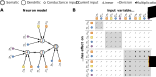
\includegraphics{media/chapters/03_nlif/03_03/nlif_product_terms.pdf}
	\caption[Effects of the relative location of input channels on the dendritic nonlinearity $H$]{Effects of the relative location of input channels on the dendritic nonlinearity $H$. \textbf{(A)}~Dendritic tree used in our example.
	The second compartment is only connected through the soma to the third and fourth compartment.
	\textbf{(B)} Table illustrating how pairs of input channels in \emph{(A)} interact according to \Cref{thm:nlif_product_terms}.
	Grey rectangles correspond to branches with nonlinear interaction.
	The symbol \enquote{$/$} indicates that $H$ only contains linear combinations of terms containing each variable; \enquote{$\div$} indicates that the variable in this column acts divisively on the other variable in the numerator; \enquote{$\bullet$} indicates that $H$ contains product terms with these two variables.}
	\label{fig:nlif_product_terms}
\end{figure}

\begin{definition}[Branch]
A \emph{branch} of an \nlif neuron is a set of compartments that form a connected component in the \nlif connectivity graph even if the somatic compartment is removed from the neuron.
\end{definition}

\begin{restatable}{theorem}{ThmNlifProductTerms}
\label{thm:nlif_product_terms}
Consider an \nlif neuron with $\ell$ branches, where each compartment is connected to $k$ unique con\-duc\-tance- and $k$ unique current-based input channels.
We denote these inputs as $g_j^i$ and $J_j^i$, where $i$ and $j$ are the compartment and input channel indices, respectively.
Furthermore, arrange the compartment indices such that $i_{m - 1} + 1, \ldots, i_{m}$ belong to the same branch, where $m$ with $1 \leq m \leq \ell$ is the branch index.
Then, the somatic current model $H$ has the following form
\begin{align*}
	H_0(g_1^1, \ldots, g_k^1, J_1^1, \ldots, J_k^1) +
	\frac{H^B_1(
		g_1^{2}, \ldots, g_k^{i_1} \!,
		J_1^{2}, \ldots, J_k^{i_1})
	}{
		H^A_1(g_1^{2}, \ldots, g_k^{i_1})
	}
	+ \ldots +
	\frac{H^B_\ell(
		g_1^{i_{\ell - 1} + 1}, \ldots, g_k^{i_\ell},
		J_1^{i_{\ell - 1} + 1}, \ldots, J_k^{i_\ell})
	}{
		H^A_\ell(g_1^{i_{\ell - 1} + 1}, \ldots, g_k^{i_\ell})
	} \,,
%	\label{eqn:nlif_product_terms}
\end{align*}
where \emph{(A)}~$H_0$ is an \emph{affine} function over all inputs injected into the somatic compartment, \emph{(B)}~the $H^A_m$ are nonnegative affine functions of product terms between conductanced-based inputs belonging to \emph{different} dendritic compartments, and \emph{(C)}~the $H^B_m$ are affine functions of product terms between conductance-based inputs belonging to \emph{different} dendritic compartments, and \emph{at most one} dendritic current-based input per product term.
\end{restatable}

\subsubsection{Affine terms}
The \enquote{computationally weakest} \nlif neurons are those where the somatic current is merely an affine function over the input channels.
As follows from \Cref{thm:nlif_product_terms}, this is the case for \nlif neurons that only possess a somatic compartment, or, more generally, any \nlif neuron where input is solely fed into the somatic compartment.
The same holds for \nlif neurons that only possess current-based input channels.

\subsubsection{Shunting}
\Cref{thm:nlif_product_terms} similarly dictates that nonlinear interaction between the input channels of an individual dendritic compartment is limited to \enquote{shunting} \citep[cf.][Section~1.5]{koch1999biophysics}.
That is, conductance-based input channels act \enquote{divisively} on the other input channels in that compartment; they contribute to the denominator of one of the fractions in \Cref{thm:nlif_product_terms}.

Mathematically, this kind of nonlinear interaction is apparent in the dendritic nonlinearity for the two-compartment neuron (eq.~\ref{eqn:two_comp_lif}); the excitatory and inhibitory conductances $g_\mathrm{E}$ and $g_\mathrm{I}$ act divisively on $H$.
While the magnitude of this effect depends on the ratio between the input and the coupling- and leak-conductances, shunting in a single compartment cannot be used to compute \enquote{interesting} functions such as \XOR (proof in \Cref{app:thm_two_comp_xor}):
\begin{restatable}{theorem}{ThmTwoCompXor}
\label{thm:two_comp_xor}
Let $g_\mathrm{E}(x_1, x_2) = g_\mathrm{E}^1(x_1) + g_\mathrm{E}^2(x_2)$ and $g_\mathrm{I}(x_1, x_2) = g_\mathrm{I}^1(x_1) + g_\mathrm{E}^2(x_2)$ be nonnegative functions.
Furthermore, let $a_0 > 0$ and $a_1, a_2, b_0, b_1, b_2 \geq 0$.
The two-compartment \LIF nonlinearity
\begin{align*}
	\phi(x_1, x_2) = H(g_\mathrm{E}(x_1, x_2), g_\mathrm{I}(x_1, x_2)) &= \frac{b_0 + b_1 g_\mathrm{E}(x_1, x_2) - b_2 g_\mathrm{I}(x_1, x_2)}{a_0 + a_1 g_\mathrm{E}(x_1, x_2) + a_2 g_\mathrm{I}(x_1, x_2)}
\end{align*}
cannot be used to solve the weak \XOR problem (see \Cref{def:weak_xor}).
\end{restatable}

Still, and as we demonstrate in the next section, a single layer of two-compartment neurons can compute a wide range of functions with a substantially smaller error than a single layer, or, in some cases, even two layers of standard \LIF neurons.

\subsubsection{Product terms}
Input channels targeting different dendritic compartments interact multiplicatively (cf. eq.~\ref{eqn:three_comp_lif_long}).
%As we discussed above, multiplication over all four quadrants in $[-1, 1]^2$ can be interpreted as a continuous version of the XOR function.
However, exploiting the product terms to compute multiplication over all four quadrants is difficult for multiple reasons.
First, conductance-based inputs are nonnegative, and can thus only cover one quadrant.
While current-based channels can provide positive and negative input, there is at most one current-based input per product term.

Second, the multiplicative terms are similar in magnitude to the linear terms---for example, all terms in the numerator in \cref{eqn:three_comp_lif_long} are the product of two conductances and one voltage, whereas all terms in the denominator are the product of two conductances.
This implies that, to compute a function such as \XOR, we must find synaptic weights that compensate for the linear terms, while, at the same time, computing the desired nonlinear function.

Lastly, there is a tradeoff between the coupling conductances $c_{ij}$ and the maximum somatic current that can be produced by a compartment.
This current is proportional to the product of the intermediate coupling conductances, making it more difficult for distal compartments to influence the soma.
Countering this by choosing larger $c_{ij}$ results in more linear $H$.

Still, as we demonstrate in \Cref{sec:nlif_opt}, it is indeed possible to solve the weak \XOR problem using a single three-compartment neuron.
In particular, we discuss an iterative weight optimisation scheme that in practice quickly converges to locally optimal weights.

